\chapter{Batch Script Transformer}

This tool helps you do script transformation for multiple files at a time. This can save time if you have many Pāli text files needed the conversion. The tool is simple and straightforward. It works only with text files. You can open the transformer by menu \texttt{File>Batch Script Transformer}.

First, you have to add files by hitting the button provided, select the output script you want, then hit the \texttt{Convert} button. That is all. Figure \ref{fig:batch-script-transformer} shows the result from my playing.

\begin{figure}[!hbt]
\centering
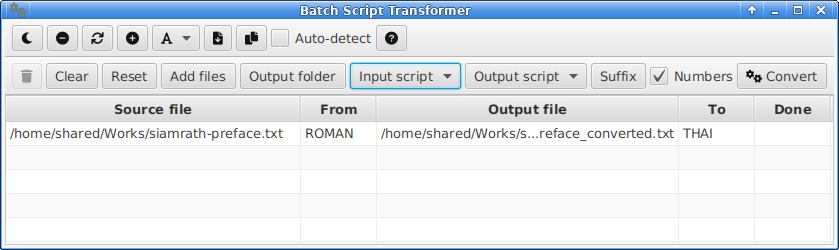
\includegraphics[width=0.9\linewidth]{images/batch-script-transformer.png}\\
\caption{Batch Script Transformer window}
\label{fig:batch-script-transformer}
\end{figure}

There are some other things you should be aware of. You can convert from Roman script to any of other scripts, but other scripts can be converted only to Roman. You can set the output folder by the button provided, otherwise you have to use suffix added to the output files' name. The default suffix is `\_converted.' You can change this by its button. You can choose whether numbers are included in the conversion or not. This option works only in the transformation from Roman to other scripts. The \texttt{Reset} button is used after a transformation is successfully done so that you can do it again, possibly with a different output script.
